%%%%%%%%%%%%%%%%%%%%%%%%%%%%%%%%%%%%%%%%%
% Short Sectioned Assignment
% LaTeX Template
% Version 1.0 (5/5/12)
%
% This template has been downloaded from:
% http://www.LaTeXTemplates.com
%
% Original author:
% Frits Wenneker (http://www.howtotex.com)
%
% License:
% CC BY-NC-SA 3.0 (http://creativecommons.org/licenses/by-nc-sa/3.0/)
%
%%%%%%%%%%%%%%%%%%%%%%%%%%%%%%%%%%%%%%%%%

%----------------------------------------------------------------------------------------
%	PACKAGES AND OTHER DOCUMENT CONFIGURATIONS
%----------------------------------------------------------------------------------------

\documentclass[paper=a4, fontsize=11pt]{scrartcl} % A4 paper and 11pt font size

\usepackage[T1]{fontenc} % Use 8-bit encoding that has 256 glyphs
%\usepackage{fourier} % Use the Adobe Utopia font for the document - comment this line to return to the LaTeX default
\usepackage[english]{babel} % English language/hyphenation
\usepackage{amsmath,amsfonts,amsthm} % Math packages
\usepackage{units}
\usepackage{hyperref}
\usepackage{lipsum} % Used for inserting dummy 'Lorem ipsum' text into the template
\usepackage{caption}

\usepackage{sectsty} % Allows customizing section commands
\allsectionsfont{\centering \normalfont\scshape} % Make all sections centered, the default font and small caps
\usepackage{amsmath}
\usepackage{fancyhdr} % Custom headers and footers
\pagestyle{fancyplain} % Makes all pages in the document conform to the custom headers and footers
\fancyhead{} % No page header - if you want one, create it in the same way as the footers below
\fancyfoot[L]{} % Empty left footer
\fancyfoot[C]{} % Empty center footer
\fancyfoot[R]{\thepage} % Page numbering for right footer
\renewcommand{\headrulewidth}{0pt} % Remove header underlines
\renewcommand{\footrulewidth}{0pt} % Remove footer underlines
\setlength{\headheight}{13.6pt} % Customize the height of the header
\usepackage{subcaption}
\numberwithin{equation}{section} % Number equations within sections (i.e. 1.1, 1.2, 2.1, 2.2 instead of 1, 2, 3, 4)
\numberwithin{figure}{section} % Number figures within sections (i.e. 1.1, 1.2, 2.1, 2.2 instead of 1, 2, 3, 4)
\numberwithin{table}{section} % Number tables within sections (i.e. 1.1, 1.2, 2.1, 2.2 instead of 1, 2, 3, 4)
\usepackage{graphicx}
\setlength\parindent{0pt} % Removes all indentation from paragraphs - comment this line for an assignment with lots of text

%----------------------------------------------------------------------------------------
%	TITLE SECTION
%----------------------------------------------------------------------------------------

\newcommand{\horrule}[1]{\rule{\linewidth}{#1}} % Create horizontal rule command with 1 argument of height

\title{	
\normalfont \normalsize 
\textsc{Michigan State University} \\ [25pt] % Your university, school and/or department name(s)
\horrule{0.5pt} \\[0.4cm] % Thin top horizontal rule
\huge  Project 2 \\ % The assignment title
\horrule{2pt} \\[0.5cm] % Thick bottom horizontal rule
}

\author{Alex Dombos, Samuel Lipschutz, Charles Loelius} % Your name

\date{\normalsize 2/5/14} % Today's date or a custom date

\begin{document}

\maketitle % Print the title

%----------------------------------------------------------------------------------------
%	PROBLEM 1
%----------------------------------------------------------------------------------------

\section{Target Selection}

In this case, we consider the setup to be a target of stable $^{58}$Ni, in its ground state. We thereby find that we have quantum numbers in the entrance partition corresponding to(assuming neutron/proton scattering):\\
\begin{center}
\begin{table}[h!]
\captionsetup{font=large}
\caption{Table of Quantum Values}
\centering
\vspace{3 mm}
\begin{tabular}{|c|c|}

Quantum Number & Value \\
Mass partition x & T=58,P=1\\
Charge & 28 \\
Spin & 0\\
Parity & +


\end{tabular}
\end{table}
\end{center}


\section{Pointlike and Structured Coulomb Scattering}

We would expect,in the absence of any nuclear forces, and for a point like nucleus, we would expect that the proton would have a pure Rutherford cross section.Upon taking into account the finite size of the target, we recognize that there is a perturbation in the distribution of charge, so that the electric potential will switch from a $\frac{1}{r}$ term to a linear term proportional to $r$. We expect that this should mean that at energies high enough to probe the structure of the proton-i.e. those that can overcome the coulomb potential to have a reasonably large wavefunction in the vicinity of the proton- there ought to be an increased cross section in the forward direction. \\

We compare this below to four graphs of the coulomb potential, one pointlike and one with spatial extent, with energies of .1 MeV and 50 MeV.\\

 \begin{figure}[hbt]
        \centering
        \begin{subfigure}[b!]{0.45\textwidth}
                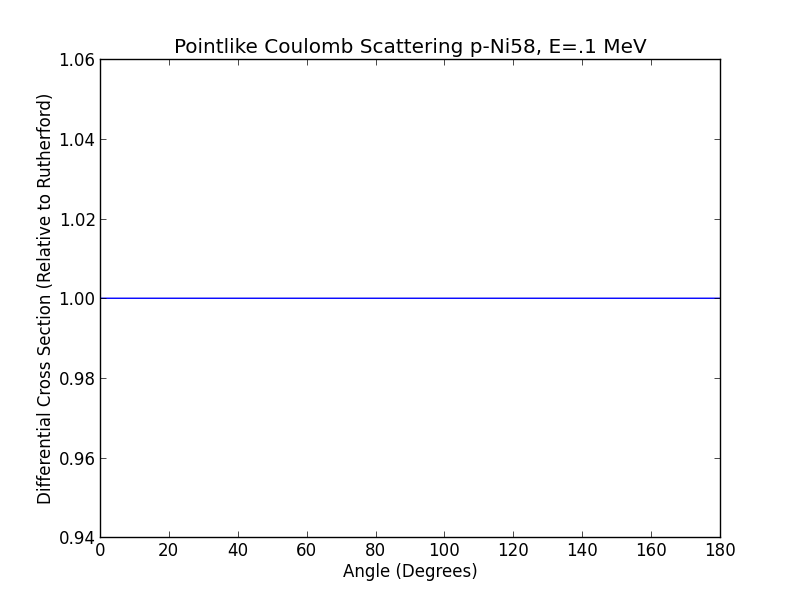
\includegraphics[width=\textwidth]{PointlikeEpoint1.png}
        \end{subfigure}%
        ~ %add desired spacing between images, e. g. ~, \quad, \qquad etc.
          %(or a blank line to force the subfigure onto a new line)
\quad
        \begin{subfigure}[b!]{0.45\textwidth}
                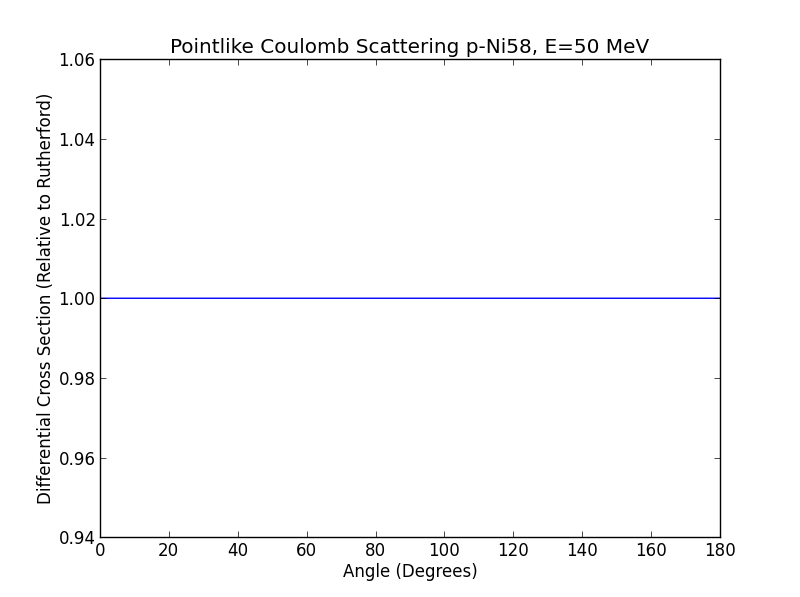
\includegraphics[width=\textwidth]{PointlikeE50.png}
        \end{subfigure}
\\
        ~ %add desired spacing between images, e. g. ~, \quad, \qquad etc.
          %(or a blank line to force the subfigure onto a new line)
        \begin{subfigure}[b]{0.45\textwidth}
                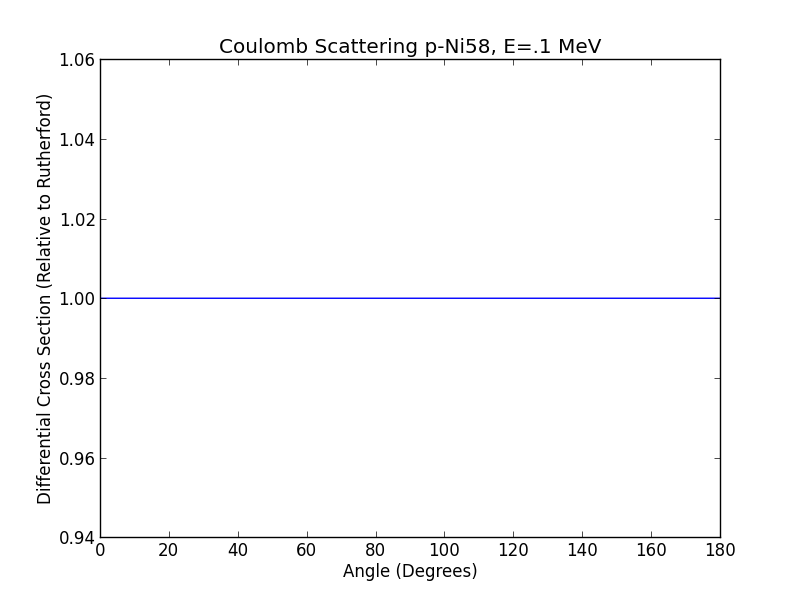
\includegraphics[width=\textwidth]{Coulombpoint1.png}
        \end{subfigure}
\quad
        \begin{subfigure}[b]{0.45\textwidth}
                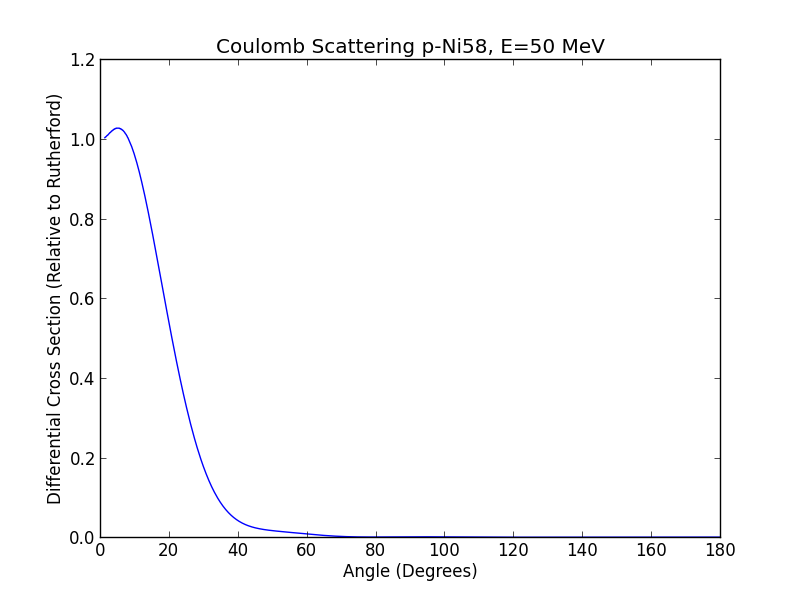
\includegraphics[width=\textwidth]{Coulomb50.png}
        \end{subfigure}

        \caption{Comparison of Pointlike (top) and Extended (bottom) Coulomb Cross Sections }
\end{figure}

We see that this is exactly what was anticipated, that the pointlike coulomb scattering is indentical to the Rutherford cross section, wheras the case where the target (Nickel 58) has a radial extent shows no structure for low energy projectiles but has the expected forward peaking for high energy. \\
\newpage
\section{Neutron-Nickel Analysis}
\subsection{Differential Cross Sections}
We then consider the previous analysis using a similar potential model for the nuclear optical potential, but setting the charge of the projectile to 0, and changing the optical potential to be for n-scattering as found at \url{https://www-nds.iaea.org/cgi-bin/ripl_om_param.pl?Z=28&A=58&ID=1417&E1=0.1&E2=150}. The results of this are plotted below.\\


 \begin{figure}[hbt]
        \centering
        \begin{subfigure}[b!]{0.45\textwidth}
                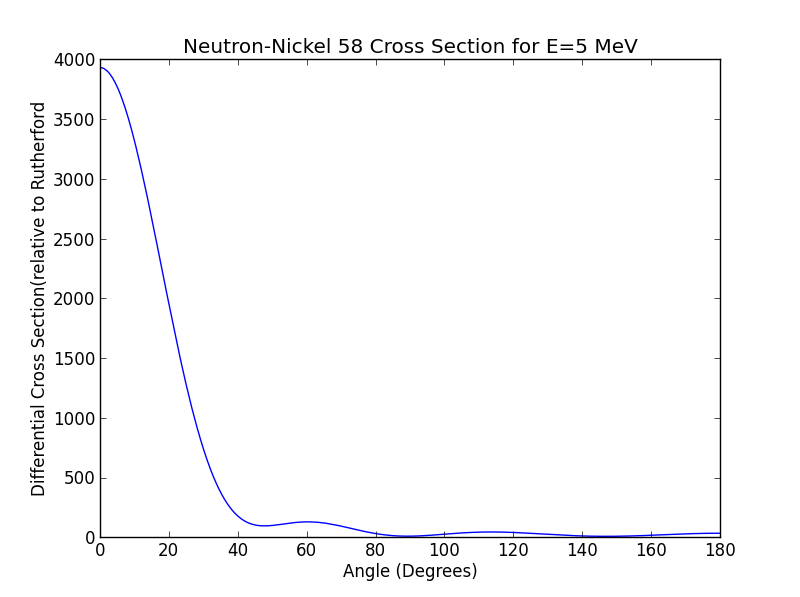
\includegraphics[width=\textwidth]{NeutronNi5.png}
        \end{subfigure}%
        ~ %add desired spacing between images, e. g. ~, \quad, \qquad etc.
          %(or a blank line to force the subfigure onto a new line)
\quad
        \begin{subfigure}[b!]{0.45\textwidth}
                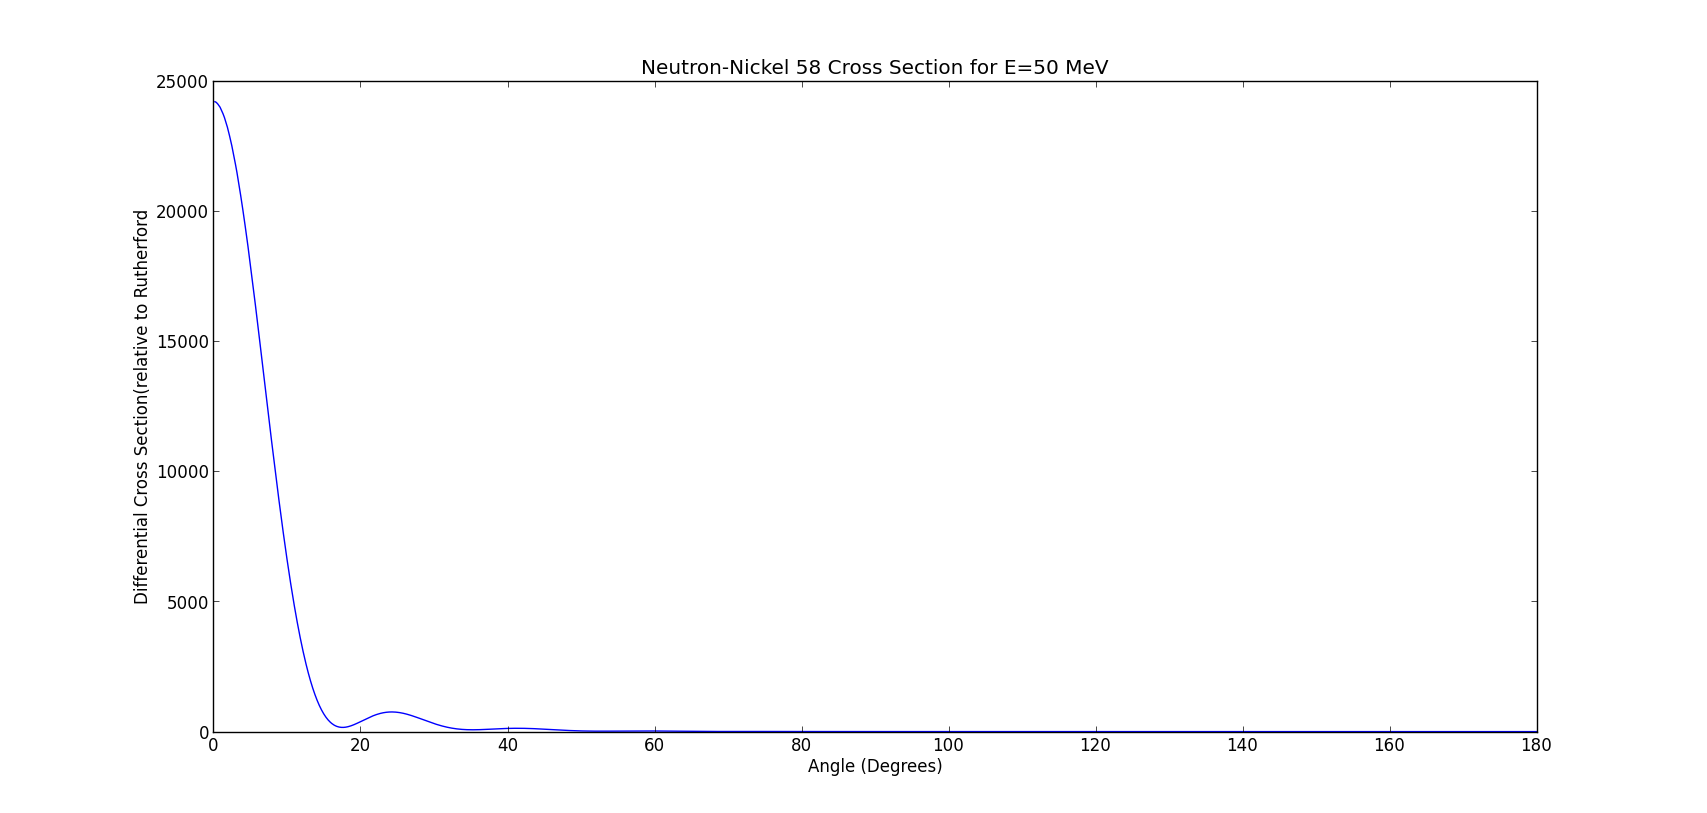
\includegraphics[width=\textwidth]{NeutronNi50.png}
        \end{subfigure}

        \caption{Differential Cross Sections for Neutron Interactions}
\end{figure}

We can see in this case that the distributions are sharply peaked near zero, with the major difference being in the extreme sharpness of the 50 MeV compared to a somewhat  broader peak for the 5 MeV. This makes sense because in the absence of a coulomb interaction, the only potential is the optical potential. Since the 50 MeV neutron has a larger energy compared to the optical potential and so is less affected. However, the 5 MeV neutron, no longer prevented from interacting with the optical potential due to the coulomb force, is likely to interact more with the optical potential. This explains the broader scattering. We might expect something similar as energy decreases and the optical potential causes further interactions. However, this must be reconciled with an expected decrease in flux caused by increase interactions with the imaginary potential.\\

\subsection{Increased Diffuseness}

In this case, I have set the diffuseness paramaeter to be ten times larger than in the standard found in the previous optical potential. This results in a cross section as follows(for 5 MeV):\\
\begin{figure}[hbt]
\centering
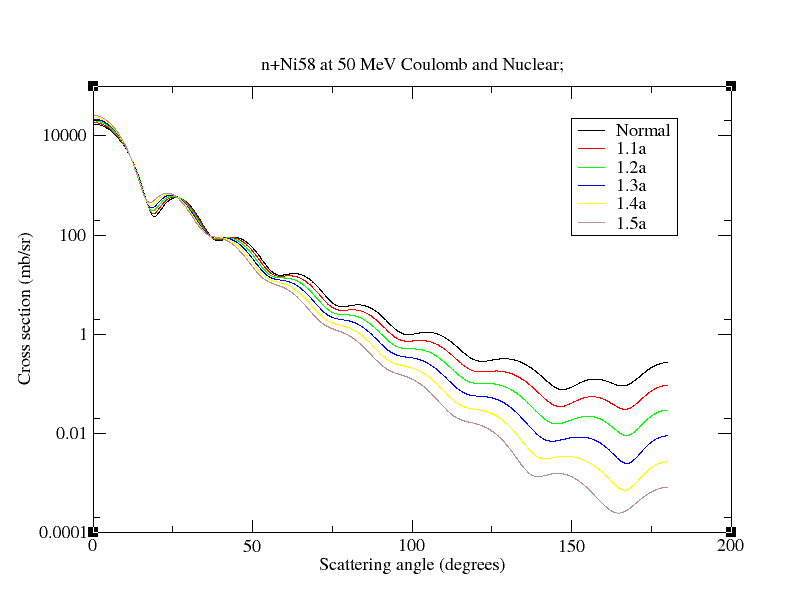
\includegraphics[width=\textwidth]{NeutronDiff.png}
\end{figure}

We see that for increased diffusiveness that the forward cross section becomes nearly infinite, in comparison to the Rutherford cross section, which follows because at a near infinitely large diffusive constant the potential is nearly zero in any area and so has no effect on the trajectory. Thus the particle will continue unperturbed, and so have a scattering angle of 0. As such it follows that this will be much larger than the Rutherford cross section which in principle should allow for no such scattering. What's more, the diffuseness means the imaginary potential absorbs less and so the cross section becomes much larger.\\


\subsection{Increased Radius}

In this case we consider a radius parameter in the optical potential to also be ten times larger than in the potential defined above. This has the effect of increasing the range over which the potential is strong, and so increases the overall effect of the potential, leaving a larger relative amount of the cross section over which to be scattered. However, it also increases the surface area and volume, which means that there is an increased probability for absorption through the imaginary potential and so an overall smaller cross section.

\begin{figure}[hbt]
\centering
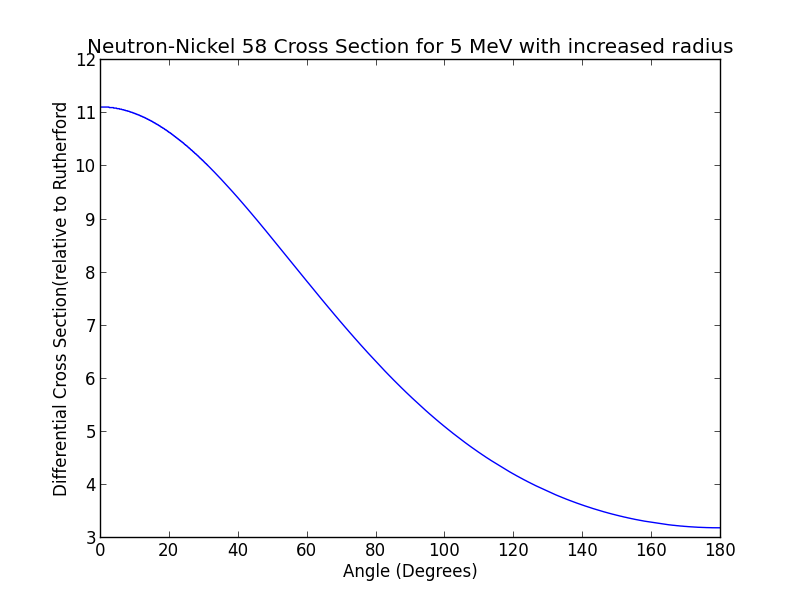
\includegraphics[width=\textwidth]{NeutronRad.png}
\end{figure}

\subsection{Different Strength of Imaginary Potentials}

We then ought to anticipate a difference in the total cross sections and so the elastic differential cross sections of the potential, and so a strong imaginary potential(in this case multiplied by ten from the above) ought to have a much smaller cross section than that of the weak potential(in this case wth the strength of the imaginary potentials divided by ten.)

These are plotted below:

 \begin{figure}[hbt!]
        \centering
        \begin{subfigure}[b!]{0.45\textwidth}
                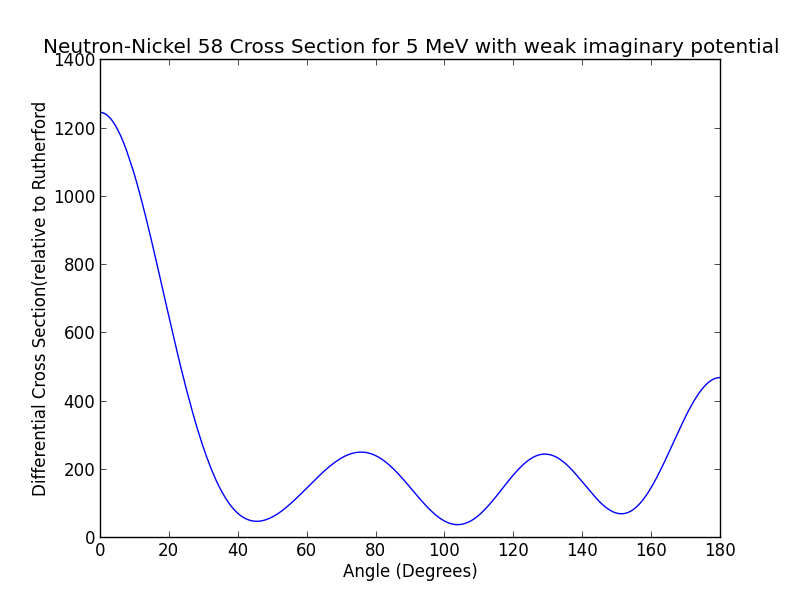
\includegraphics[width=\textwidth]{NeutronWeakcs.png}
        \end{subfigure}%
        ~ %add desired spacing between images, e. g. ~, \quad, \qquad etc.
          %(or a blank line to force the subfigure onto a new line)
\quad
        \begin{subfigure}[b!]{0.45\textwidth}
                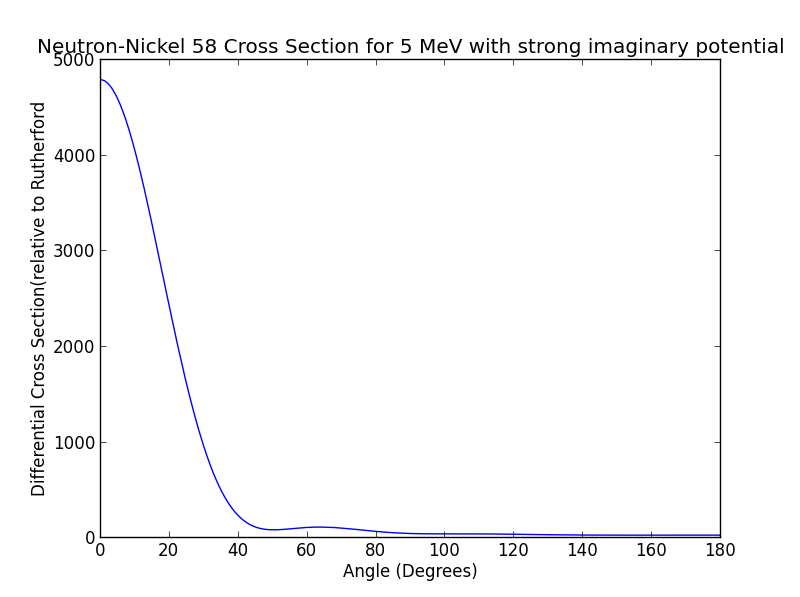
\includegraphics[width=\textwidth]{NeutronStrongcs.png}
        \end{subfigure}

        \caption{Differential Cross Sections for Neutron-Ni58 with Varying Imaginary Potentials}
\end{figure}
\newpage
We note that in this instance we don't seem to have the same agreement expected, as it would appear that there is a larger cross section with the strong imaginary potential. However, instead we should look at the modul of the S matricesi for different L states, which will show the overall absorption. These are plotted below:\\


 \begin{figure}[hbt!]
        \centering
        \begin{subfigure}[b!]{0.45\textwidth}
                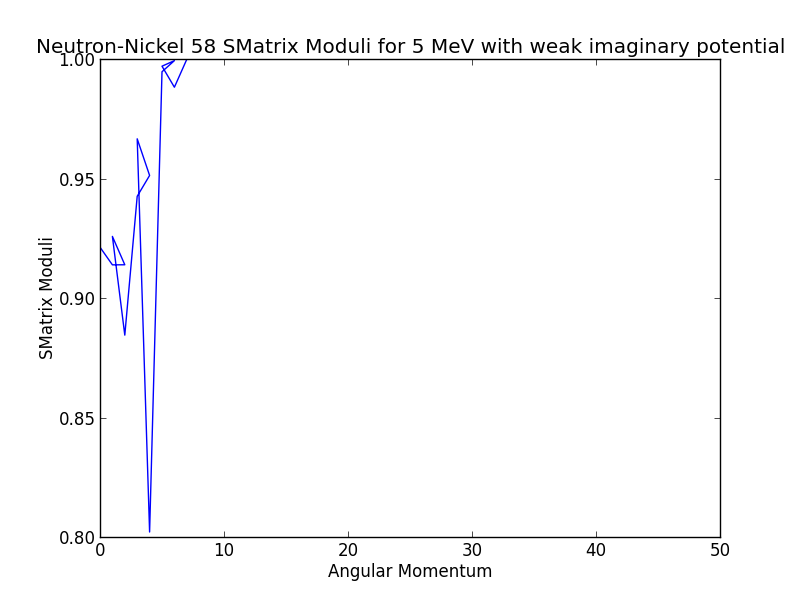
\includegraphics[width=\textwidth]{NeutronWeaks.png}
        \end{subfigure}%
        ~ %add desired spacing between images, e. g. ~, \quad, \qquad etc.
          %(or a blank line to force the subfigure onto a new line)
\quad
        \begin{subfigure}[b!]{0.45\textwidth}
                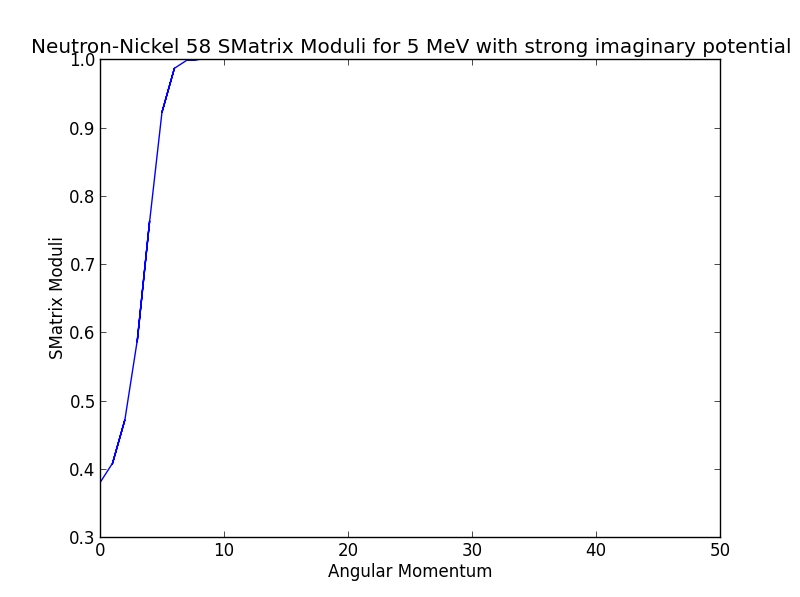
\includegraphics[width=\textwidth]{NeutronStrongs.png}
        \end{subfigure}

        \caption{Moduli of S for Neutron-Ni58 with Varying Imaginary Potentials}
\end{figure}

Here we see clearly that especially at low angular momenta the strong imagnary potential starts with a much smaller S matrix than that of the weak, and only slowly converges to 1 with a large L. \\

\section{Total Cross Sections}

We return to the five and fifty MeV neutron-Ni58 scattering previously examined, note that in the output files generated there is in fort.40 a description of the cross sections. We plot the results in the table below:\\

\begin{table}[hbt!]
\centering
\begin{tabular}{|c|c|c|c|}
Energy(MeV) & Reaction Cross Section & Elastic Cross Section& Total Cross Section\\
5 & 2262 & 1802 & 4064 \\
50 & 1548 &1889 & 3437 
\end{tabular}
\caption{Table of Cross Sections}
\end{table}

And in this we see that the high energy neutron has a lower overall cross section, primarily driven by an increased lack of reactions as the potential is unable to affect the high energy neutron much.

\end{document}
